\documentclass[12font]{article}
\title{\textbf{ How to Get the Correct Area Law }}
\author{Chen-Chih Wang  }
\date{\textit{Department of physics, National Tsing Hua University, Hsinchu 30013, Taiwan} \\ (Dated: \today)}
\usepackage[margin=2cm]{geometry}
%\usepackage[fleqn]{amsmath}
%\usepackage{CJK,amsmath}
\usepackage{amsfonts,amssymb}
\usepackage{fancyhdr}
%\pagestyle{fancy}
\usepackage{textcomp}
\usepackage{graphicx}
\usepackage{float}
\usepackage{color}
\usepackage{tikz}
\usepackage{multicol}
\usepackage{threeparttable}
\usepackage{amsthm}
\usepackage{mathtools}
\usepackage{hyperref}
\urlstyle{same}
\usepackage{caption}
\usepackage{subcaption}
\usepackage{dsfont}

\newcommand{\vac}{\mrm{vac}}
\newcommand{\Bra}[1]{\left\langle #1 \right|}
\newcommand{\Ket}[1]{\left| #1 \right\rangle}
\newcommand{\bra}[1]{\langle #1 |}
\newcommand{\ket}[1]{| #1 \rangle}
\newcommand{\anglelr}[1]{\left\langle #1 \right\rangle}
\newcommand{\braket}[2]{\langle #1 | #2 \rangle}
\newcommand{\Bbraket}[2]{\left\langle #1 \right|\left. #2 \right\rangle}
\newcommand{\dif}[1]{\frac{\mathrm{d}}{\mathrm{d}#1}}
\newcommand{\diff}[2]{\frac{\mathrm{d}#1}{\mathrm{d}#2}}
\newcommand{\gd}{\boldsymbol{\nabla}}
\newcommand{\dive}{\boldsymbol{\nabla}\cdot}
\newcommand{\curl}{\boldsymbol{\nabla}\times}
\newcommand{\lr}[1]{\left(  #1  \right)}
\newcommand{\lrm}[1]{\left[  #1  \right]}
\newcommand{\lrg}[1]{\left\{  #1  \right\}}
\newcommand{\abs}[1]{\left|  #1  \right|}
\newcommand{\de}{\partial}
\newcommand{\pdif}[1]{\frac{\partial}{\partial#1}}
\newcommand{\pdifn}[2]{\frac{\partial^#2}{\partial#1^#2}}
\newcommand{\pdiff}[2]{\frac{\partial#1}{\partial#2}}
\newcommand{\pdiffn}[3]{\frac{\partial^#3 #1}{\partial#2^#3}}
\newcommand{\mrm}[1]{\mathrm{#1}}
\newcommand{\bo}[1]{\mathbf{#1}}
\newcommand{\bog}[1]{\boldsymbol{#1}}
\newcommand{\vint}[3]{\int_{#1}#2\cdot\mathrm{d}\mathbf{#3}}
\newcommand{\voint}[3]{\oint_{#1}#2\cdot\mathrm{d}\mathbf{#3}}
\newcommand{\Vint}{\int\mrm{d}^3\bo{r}'}
\newcommand{\rr}{\mathbf{r} - \mathbf{r}'}
\newcommand{\arr}{\left|\mathbf{r} - \mathbf{r}'\right|}
\newcommand{\nx}{\hat{\bo{n}}_1}
\newcommand{\ny}{\hat{\bo{n}}_2}
\newcommand{\alert}[1]{{\color{red}#1}}
\newcommand{\alertV}[1]{{\color{violet}#1}}
\newcommand{\Tr}{\mrm{Tr}}
\newcommand{\norm}[1]{\left\lVert#1\right\rVert}
\newcommand{\dimer}[2]{\sigma^{\alpha_{#1 #2}}_{#1}\sigma^{\alpha_{#1 #2}}_{#2}}

\newcommand{\wordfig}[2]{\begin{minipage}[h]{#1 cm}
	\vspace{0pt}
	\includegraphics[width=\textwidth]{#2}
   \end{minipage}}
   
\begin{document}

\maketitle

To simplify the discussion, I will restrict myself to cases with an even number of sites.

As we know, the area law entanglement entropy of a chosen geometric region $A$ with $n$ disconnected boundaries reads
\[
S_A \sim \alpha \abs{\de A} - n\gamma
\]
where $\gamma$ is the topological entanglement entropy. 
\section{Simply-connected cases}
In the Kitaev model, the \textit{entanglement spectral degeneracy} is responsible for the topological term. Consider a \textbf{simply-connected} $A$, and according to our finding, the Majorana representation of the reduced density matrix reads
\begin{equation}\label{equ.rho_F}
    \rho_A^F = \frac{1}{2^{N^A/2}}\sum_{[\mathcal{M}]\subset A}\mathfrak{C}_\mathcal{M}V_{\mathcal{M}}
\end{equation}
where $V_\mathcal{M} := \prod_{\anglelr{ij}\in\mathcal{M}}ic_ic_j$; While the spin representation of the reduced density matrix reads
\begin{equation}\label{equ.rho}
    \rho_A = \frac{1}{2^{N^A-N^A_p}}\sum_{[\mathcal{M}]\subset A}\mathfrak{C}_\mathcal{M}U_{\mathcal{M}}
\end{equation}
where
\[
U_\mathcal{M} := \prod_{p\in A}\lr{\frac{\mathds{1} + W_p}{2}}\prod_{\anglelr{ij}\in \mathcal{M}}\dimer{i}{j}
\]
A convenient property we can take advantage of is that the algebra of $U$ and $V$ are identical
\[
\left\{
\begin{aligned}
& U_\mathcal{M}U_{\mathcal{M'}}=g(\mathcal{M},\mathcal{M}')U_{\mathcal{M}\oplus\mathcal{M}'} \\
& V_\mathcal{M}V_{\mathcal{M'}}=g(\mathcal{M},\mathcal{M}')V_{\mathcal{M}\oplus\mathcal{M}'}
\end{aligned}
\right.
\]
And we also know that 
\[
\left\{
\begin{aligned}
&\Tr U_{\mathcal{M}} = 2^{N^A-N^A_p}\delta_{\mathcal{M},\varnothing} \\
& \Tr_F V_{\mathcal{M}} = 2^{N^A/2}\delta_{\mathcal{M},\varnothing}
\end{aligned}
\right.
\]
where $\Tr_F$ stands for taking trace over the Majorana fermion space in the region $A$. Therefore, for an arbitrary analytical function $f$, we have an identity:
\begin{equation}\label{equ.identity}
    \Tr f(\lrg{U}) = \frac{1}{2^{N^A/2 - N^A_p}}\Tr_F f(\lrg{V})
\end{equation}

In light of this, define a function
\[
f(\lrg{W}) \equiv \lrm{\frac{1}{2^{N^A-N^A_p}}\sum_{[\mathcal{M}]\subset A}\mathfrak{C}_\mathcal{M}W_{\mathcal{M}}}\ln\lrm{\frac{1}{2^{N^A-N^A_p}}\sum_{[\mathcal{M}]\subset A}\mathfrak{C}_\mathcal{M}W_{\mathcal{M}}}
\]
and hence
\[
\left\{
\begin{aligned}
&\rho^F_A\ln\rho_A^F = \frac{1}{2^{N^A/2-N^A_p}} f\lr{\lrg{V}} - \lrm{\lr{N^A/2-N^A_p}\ln 2}\rho^F_A \\
& \rho_A\ln\rho_A = f\lr{\lrg{U}}
\end{aligned}
\right.
\]
And the entanglement entropy is then
\begin{equation}\label{equ.simple_result}
    S_A = -\Tr f(\lrg{U}) = -\frac{1}{2^{N^A/2 - N^A_p}}\Tr_F f(\lrg{V}) = \underbrace{-\Tr_F \rho^F_A\ln\rho^F_A}_{S^F_A} + \lr{\frac{N^A}{2}-N^A_p}\ln 2 = S^F_A + \underbrace{\lr{\frac{1}{2}\abs{\de A}-1}\ln 2}_{S^G_A}
\end{equation}
where we have used the relation
\begin{equation}\label{equ.Pick}
    \abs{\de A} = N^A - 2N^A_p + 2
\end{equation}
We see that the method works perfectly well. However, the method needs to be modified a little bit when it comes to the regions with multiply-connected regions.

\section{Multiply-connected cases}
Now the question is: \textbf{\textit{How to get the correct topological term if $A$ is a multiply-connected region?}} We anticipate that the scaling of the gauge-part entanglement entropy will become
\begin{equation}\label{equ.anticipation}
    S_A^G = \frac{\ln 2}{2}\abs{\de A} - \lr{g+1}\ln 2
\end{equation}
where $g$ is the genus number of $A$. Different from the previous cases (\ref{equ.Pick}), the relation between the number of sites and the circumference becomes
\[
\abs{\de A} = N^A - 2N^A_p + 2\lr{1-g}
\]
Now we do the reverse engineering and see what form the reduced density matrix should be to give an answer satisfying our anticipation. I expect that there should be an additional projector $\mathcal{P}^{(h)}$, which commutes with every component of the density matrix $[\mathcal{P}^{(h)},U_\mathcal{M}]\forall\mathcal{M}$, to project out $2g$ dimensions. That is to say, the reduced density matrix is anticipated to be of the form
\[
\rho_A =  \frac{1}{2^{-2g}}\mathcal{P}^{(h)} \frac{1}{2^{N^A-N^A_p}} \sum_{[\mathcal{M}]\subset A}\mathfrak{C}_\mathcal{M}U_{\mathcal{M}} \to \frac{1}{2^{N^A-N^A_p-2g}}\sum_{[\mathcal{M}]\subset A}\mathfrak{C}_\mathcal{M}U'_{\mathcal{M}}
\]
where I define a new representation $U'_\mathcal{M}:= \mathcal{P}^{(h)}U_\mathcal{M}$ obeying the same algebra as $U$. With this additional projection, the relations we have met earlier become
\[
\left\{
\begin{aligned}
&\Tr U'_{\mathcal{M}} = 2^{N^A-N^A_p-2g}\delta_{\mathcal{M},\varnothing} \\
& \Tr_F V_{\mathcal{M}} = 2^{N^A/2}\delta_{\mathcal{M},\varnothing}
\end{aligned}
\right.
\]
and so
\begin{equation}\label{equ.identity_2}
    \Tr f(\lrg{U'}) = \frac{1}{2^{N^A/2 - N^A_p-2g}}\Tr_F f(\lrg{V})
\end{equation}
Similarly, define a function 
\[
f(\lrg{W}) \equiv \lrm{\frac{1}{2^{N^A-N^A_p-2g}}\sum_{[\mathcal{M}]\subset A}\mathfrak{C}_\mathcal{M}W_{\mathcal{M}}}\ln\lrm{\frac{1}{2^{N^A-N^A_p-2g}}\sum_{[\mathcal{M}]\subset A}\mathfrak{C}_\mathcal{M}W_{\mathcal{M}}}
\]
and hence
\[
\left\{
\begin{aligned}
&\rho^F_A\ln\rho_A^F = \frac{1}{2^{N^A/2-N^A_p-2g}} f\lr{\lrg{V}} - \lrm{\lr{N^A/2-N^A_p-2g}\ln 2}\rho^F_A \\
& \rho_A\ln\rho_A = f\lr{\lrg{U'}}
\end{aligned}
\right.
\]
Ultimately, the entanglement entropy is
\[
S_A = \frac{1}{2^{N^A/2 - N^A_p-2g}}\Tr_F f(\lrg{V}) = S_A^F + \underbrace{\lr{\frac{N^A}{2}-N^A_p-2g}\ln 2}_{S^G_A}
\]
So the gauge part of the entanglement entropy is then
\[
S^G_A = \lr{\frac{N^A}{2}-N^A_p-2g}\ln 2 = \lr{\frac{1}{2}\abs{\de A}- \lr{1-g} - 2g}\ln 2 = \frac{\ln 2}{2}\abs{\de A} - \lr{g+1}\ln 2
\]
which reproduces our expectation (\ref{equ.anticipation}).

The above demonstration tells us that \textbf{we have to find a projector $\mathcal{P}^{(h)}$ to project out extra $2g$ dimensions.} One possibility is that there exist \textbf{two $\mathbb{Z}_2$ operators, $\mathcal{L}_e$ and $\mathcal{L}_m$, for each hole in the region $A$}, such that the projector is constructed in the following way
\[
\mathcal{P}^{(h)} = \prod_{n=1}^{g}\lr{\frac{\mathds{1}+\mathcal{L}_e^{(n)}}{2}}\lr{\frac{\mathds{1}+\mathcal{L}_m^{(n)}}{2}}
\]
In light of the toric code model, the two $\mathbb{Z}_2$ operators $\mathcal{L}_e$ and $\mathcal{L}_m$ possibly correspond to the non-contractable $e$- and $m$-anyon loops of each hole. 

\section{Why we need terms additional to $W$'s}
The first reason for this question is straightforward. If we only consider the non-contractable loops that consist of only $W$'s, then there is only one type of $\mathcal{Z}_2$ operators we can find for the projector. Such an $\mathbb{Z}_2$ operators is nothing but the loop enclosing the $n$-th hole in the region $A$
\[
\mathcal{L}_W^{(n)} = \prod_{\anglelr{ij}\in \mathcal{C}^{(n)}\subset A}\dimer{i}{j}
\]
And the projector is then 
\[
\mathcal{P}^{(h)} = \prod_{n=1}^{g}\lr{\frac{\mathds{1}+\mathcal{L}_W^{(n)}}{2}}
\]
However, this projector can only project out $g$ dimensions, and thus is not sufficient to give the result we anticipated in the last section.

\begin{figure}
    \centering
    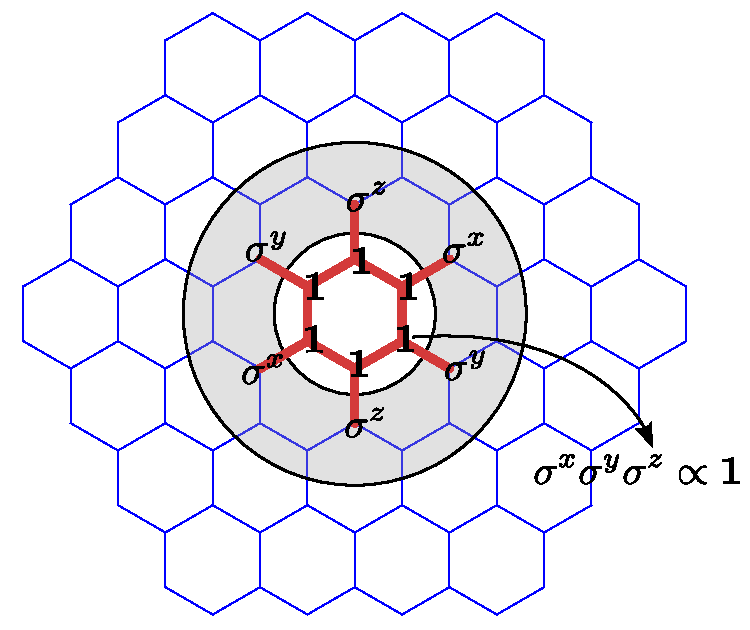
\includegraphics[width=0.4\linewidth]{hole-residual.pdf}
    \caption{The operator $\Omega^{(n)} = \Sigma_{\mathfrak{H}^{(n)}}$ is a string operator of the edge configuration $\mathfrak{H}^{(n)} \equiv h^{(n)}\cup \de h^{(n)}$. Although the edge configuration is not exclusively inside the region $A$, the Pauli operators inside the hole cancel each other to get identities all over the sites in the hole, thus the remaining spin operators are inside the region $A$, therefore, we ultimately confirm that $\Omega^{(n)}$ is a component of the reduced density matrix $\rho_A$.}
    \label{fig.hole-residual}
\end{figure}
Another reason is more subtle. If investigating the Kitaev model in detail, one will observe that there is one non-trivial type of operator that should be included in the reduced density matrix, but the form (\ref{equ.rho}) doesn't include it. Such a type of operator is one \textbf{with one $c$-Majorana fermion on every single lattice site in a hole}. I will explain this in the following.

Consider a subregion $A$ with $g=1$, as the shaded region illustrated in the equation below, an $\mathbb{Z}_2$ operator $\Omega^{(n)}$ corresponding to the $n$-th hole can be defined.
\begin{equation}\label{equ.inside-operator-def}
    \Omega^{(n)} = \Sigma_{\mathfrak{H}^{(n)}} := \prod_{\anglelr{ij}\in h^{(n)}\cup \de h^{(n)}}\dimer{i}{j} = \wordfig{3}{hole-residual-1}
\end{equation}
where the edge configuration $\mathfrak{H}^{(n)}\equiv h^{(n)}\cup\de h^{(n)}$ and $h^{(n)}$ is the set of edges in the $n$-th hole. Of course, the genus number is $g=1$ in this example, so there is only one such operator, but there will be in general more than one $\Omega$ operator if the genus number gets larger.  So what is so special about such an operator? We can see that it survives after tracing over the environment because the spin operators inside the hole cancel each other to identity as explained in Fig.\ref{fig.hole-residual}, and the remaining part lies exclusively inside the region $A$, which means it should be included in the reduced density matrix $\rho_A$. Not only this operator, whatever edge configuration $\Sigma_\mathcal{M}$ with the form $\mathcal{M}=\mathfrak{H}^{(n)}\oplus\mathcal{M}'$, where $\mathcal{M}'\subset A$. The two following equations give two examples.
\begin{align*}
    \rho_A \supset \prod_{p\in\mathfrak{P}\cap \lr{h^{(n)}\cup\de h^{(n)}}}W_p\prod_{\anglelr{ij}\in\mathcal{M}_Z\cap \lr{h^{(n)}\cup \de h^{(n)}}}\dimer{i}{j} &= \wordfig{3}{hole-residual-z-dimer} \\
    &= \underbrace{\wordfig{3}{hole-residual-1}}_{\mathfrak{H}^{(n)}} \oplus \underbrace{\wordfig{3}{hole-residual-2}}_{\subset A}
\end{align*}
\begin{align*}
    \rho_A \supset \prod_{p\in\mathfrak{S}\cap \lr{h^{(n)}\cup\de h^{(n)}}}W_p\prod_{\anglelr{ij}\in\mathcal{M}_Z \cap \lr{h^{(n)}\cup \de h^{(n)}}}\dimer{i}{j} &= \wordfig{3}{hole-residual-z-dimer-another} \\
    &= \underbrace{\wordfig{3}{hole-residual-1}}_{\mathfrak{H}^{(n)}} \oplus \underbrace{\wordfig{3}{hole-residual-2-another}}_{\subset A}
\end{align*}

However, unlike plaquette operators $W$'s, the expectation value of these $\mathbb{Z}_2$ operators $\Omega^{(n)}$ are not unity: $\anglelr{\Omega^{(n)}}\neq 1$, so it cannot be factorized out to give a projector, like the projector $\mathcal{L}_W$ did. This is the main problem I was trying to convey.


\end{document}